\documentclass[tikz,border=2pt]{standalone}
\usepackage{amsmath}
\usepackage{newtxtext,newtxmath} % Times-like to match IEEEtran
\usetikzlibrary{arrows.meta,positioning,calc,fit,shapes.multipart,decorations.pathmorphing}
\tikzset{>=Latex, line/.style={line width=0.8pt}, 
         box/.style={draw, rounded corners=2pt, minimum width=28mm, minimum height=12mm, align=center},
         note/.style={font=\footnotesize}}

\begin{document}
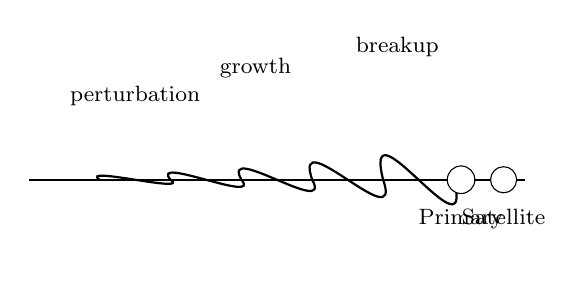
\begin{tikzpicture}[x=0.9cm,y=0.9cm]
  % Jet axis
  \draw[line] (0,0) -- (7,0);

  % Wavy breakup path
  \foreach \x/\a in {1/0.2,2/0.35,3/0.55,4/0.85,5/1.2}{
    \draw[line] (\x,0) .. controls +(-0.3,\a) and +(0.3,-\a) .. (\x+1,0);
  }

  % Labels (perturbation, growth, breakup)
  \node[note,above] at (1.5,0.9) {perturbation};
  \node[note,above] at (3.2,1.3) {growth};
  \node[note,above] at (5.2,1.6) {breakup};

  % Primary drop
  \node[draw,circle,minimum size=3.5mm,fill=white] (pri) at (6.1,0) {};
  \node[below=2pt of pri] {\footnotesize Primary};

  % Satellite drop
  \node[draw,circle,minimum size=3.0mm,fill=white] (sat) at (6.7,0) {};
  \node[below=2pt of sat] {\footnotesize Satellite};
\end{tikzpicture}
\end{document}
